\documentclass[11pt,a4paper]{article}

\usepackage[T1]{fontenc}
\usepackage[utf8]{inputenc}
\usepackage{lmodern}
\usepackage[margin=2.2cm]{geometry}
\usepackage{amsmath,amssymb}
\usepackage{booktabs}
\usepackage{tabularx}
\usepackage{array}
\usepackage{xcolor}
\usepackage{enumitem}
\usepackage{tikz}
\usetikzlibrary{positioning,arrows.meta}
\usepackage[colorlinks=true,linkcolor=blue!50!black,urlcolor=blue!50!black]{hyperref}

\newcommand{\var}[1]{\texttt{#1}}
\newcommand{\code}[1]{\texttt{#1}}
\newcolumntype{L}{>{\raggedright\arraybackslash}X}
\setlist{itemsep=2pt,topsep=4pt}

\title{Adding sectoral emission-intensity pathways\\to the v1 scenario projection}
\author{}
\date{October 2026 --- working note}

\begin{document}
\maketitle

\begin{abstract}
The v1 projection balances the EXIOBASE intermediate-flow matrix under an NGFS
short-term output scenario and a per-sector cut in embodied emissions, while
holding direct emission intensities at their 2021 level. This note sets out how
to replace that assumption with projected, sector-specific intensities. The
NGFS Phase~V long-term scenarios supply the sectoral shape of decarbonisation,
and the NGFS short-term (GEM-E3) scenarios supply output and the regional
emission level. It covers the data, the scenario and sector mappings, the
combination formula, a double-counting issue in the power sector, the changes
v1 needs and the decisions still open. Nothing described here is implemented
yet; the figures come from exploratory computations on the data in the
repository.
\end{abstract}

\tableofcontents

%=============================================================================
\section{Starting point: v1 and the intensity hook}
%=============================================================================

v1 starts from the 2021 EXIOBASE table (product-by-product, $n=200$ sectors at
the default \code{world} resolution) and the NGFS short-term output
projection $x' = x^{T,k}$. It then:
\begin{enumerate}
  \item builds the unchanged-technology counterfactual $Z_0 = A\,\mathrm{diag}(x')$
        and its column margins $v_0 = \mathbf{1}^\top Z_0$;
  \item imposes $\sum_i Z'_{ij} = v_{0,j}$ (input budgets) and
        $\sum_i s'_i Z'_{ij} = \beta_j\, b_j$ with $b_j = \sum_i s_i Z_{ij}$
        (embodied emissions of purchases, base year);
  \item solves for $Z'$ with KRAS, starting from $Z_0$, and closes the accounts
        with $A' = Z'\mathrm{diag}(x')^{-1}$ and $y' = x' - Z'\mathbf{1}$.
\end{enumerate}

Assumption H3 sets $s' = s$: intensities are frozen. The code already accepts
a projected vector, \code{project(\dots, s\_target=\dots)}, which is passed to
the constraint builder and used for the left-hand side of the emission rows,
the normalisation, the feasible band, the multipliers and the footprint
identity. What is missing is something that produces $s'$, plus a few places
that implicitly assume $s' = s$ (Section~\ref{sec:v1changes}).

%=============================================================================
\section{Data available}
%=============================================================================

\begin{table}[h]
\centering\footnotesize
\begin{tabularx}{\textwidth}{@{}lLL@{}}
\toprule
 & \textbf{NGFS short term (GEM-E3, 2025)} & \textbf{NGFS Phase V (IAMs)} \\
\midrule
Horizon, step & 2021--2030, annual & 2020--2100, 5-year nodes \\
Scenarios & Baseline, DAPS, DIRE, HWTP, SWUC & Current Policies, NDCs, Fragmented World,
  Delayed transition, Below 2\,°C, Net Zero 2050, Low demand \\
Output & \var{Production|<sector>}, 50 sectors $\times$ 60 regions, bn US\$2017 (constant prices) &
  physical only: \var{Production|Steel/Cement/Chemicals/Non-ferrous metals}, Mt/yr \\
Emissions & \var{Gross Emissions|CO2 energy, CO2 process, GHG, \dots}, Mt/yr,
  \textbf{by region only} & \var{Emissions|CO2|Energy|Demand|Industry|Steel}, \dots, Mt CO$_2$/yr,
  \textbf{by sector} \\
Energy & --- & \var{Final Energy|<sector>}, \var{Secondary Energy|Electricity}, EJ/yr \\
GDP & \var{GDP}, bn US\$2017/yr & \var{GDP|MER}, \var{GDP|PPP}, bn US\$2010/yr \\
Deflators & none in GEM-E3; EIRIN \var{Price Level|Index} (2019\,=\,1), 5 macro-regions &
  none in IAMs; NiGEM \var{Inflation rate} (\%) \\
Value added & none & none \\
Native intensities & none & none \\
\bottomrule
\end{tabularx}
\caption{What each source offers for an intensity pathway.}
\label{tab:data}
\end{table}

Two consequences follow:
\begin{itemize}
  \item Only Phase~V can tell sectors apart. GEM-E3 emissions are regional
        totals.
  \item Monetary units (US\$2010, US\$2017, current M\,EUR in EXIOBASE) and
        physical units never need to meet, provided only \emph{ratios over
        time} are transferred to EXIOBASE.
\end{itemize}
Useful conversions for ratios: Mt\,CO$_2$/bn\,US\$ $=$ kg\,CO$_2$/US\$;
Mt\,CO$_2$/Mt $=$ t\,CO$_2$/t; Mt\,CO$_2$/EJ $=$ kg\,CO$_2$/GJ, $\times 3.6$
for g\,CO$_2$/kWh.

\paragraph{Data caveat.} On GEM-E3's 8 aggregate regions (including World),
\var{Gross Emissions|GHG} and \var{Population} are labelled
``billion US\$2017''. The values show these are Mt\,CO$_2$e (46\,787 in 2021)
and million people (8\,027).

%=============================================================================
\section{Method}
%=============================================================================

\subsection{Principle}

\begin{center}
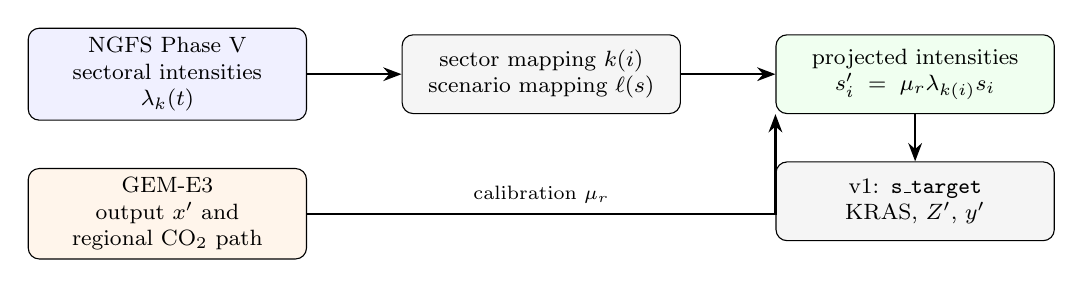
\begin{tikzpicture}[
  box/.style={draw,rounded corners,align=center,font=\footnotesize,minimum height=1.0cm,text width=3.3cm},
  arr/.style={-{Stealth},thick}]
  \node[box,fill=blue!6] (lt) {NGFS Phase V\\sectoral intensities\\$\lambda_k(t)$};
  \node[box,fill=orange!8,below=0.6cm of lt] (st) {GEM-E3\\output $x'$ and\\regional CO$_2$ path};
  \node[box,fill=gray!8,right=1.2cm of lt] (map) {sector mapping $k(i)$\\scenario mapping $\ell(s)$};
  \node[box,fill=green!6,right=1.2cm of map] (s) {projected intensities\\$s'_i = \mu_r \lambda_{k(i)} s_i$};
  \node[box,fill=gray!8,below=0.6cm of s] (v1) {v1: \code{s\_target}\\KRAS, $Z'$, $y'$};
  \draw[arr] (lt) -- (map);
  \draw[arr] (map) -- (s);
  \draw[arr] (st.east) -| node[pos=0.25,above,font=\scriptsize]{calibration $\mu_r$} (s.south west);
  \draw[arr] (s) -- (v1);
\end{tikzpicture}
\end{center}

Each source does what it can do. Phase~V gives \emph{which sectors decarbonise
and how fast}. GEM-E3 gives \emph{output} (already in v1) and \emph{the
regional emission level}. For EXIOBASE product $i$ in region $r$, short-term
scenario $s$ and year $t$:
\begin{equation}
  s'_i(t) \;=\; \mu_r(t)\;\lambda^{\ell(s)}_{k(i)}(t)\; s_i(2021),
  \label{eq:main}
\end{equation}
where
\begin{itemize}
  \item $k(i)$ is the intensity group of product $i$ (Section~\ref{sec:sectors});
  \item $\ell(s)$ is the Phase~V scenario paired with short-term scenario $s$
        (Section~\ref{sec:scenarios});
  \item $\lambda$ is a unit-free intensity ratio;
  \item $\mu_r$ is an optional regional calibration factor (Section~\ref{sec:calib}).
\end{itemize}

\subsection{Sectoral intensity ratios}

For group $k$, the Phase~V intensity is emissions over the best available
activity measure,
\begin{equation}
  I_k(t) = \frac{E_k(t)}{Q_k(t)}, \qquad
  \lambda_k(t) = \frac{I_k(t)}{I_k(2021)},
\end{equation}
where $Q_k$ is physical output where it exists (steel, cement), electricity
generation for power, and final energy otherwise. Final energy measures only
the carbon content of energy, so it is a conservative choice. The default is
the median over the three IAMs (GCAM, MESSAGE, REMIND), with the min--max
range kept as a sensitivity.

\subsection{Time interpolation}

Phase~V has nodes in 2020, 2025 and 2030. The base year is interpolated
linearly, $I(2021) = 0.8\,I(2020) + 0.2\,I(2025)$; intermediate years
2022--2030 are interpolated log-linearly between nodes. 2020 is a COVID year,
which depresses emission \emph{levels}; intensities are much less affected,
which is one more reason to transfer intensities rather than levels.

\subsection{Regional calibration to the short term}
\label{sec:calib}

$\mu_r$ makes region $r$'s projected emissions follow GEM-E3's CO$_2$ growth
(\var{CO2 energy} $+$ \var{CO2 process}, which matches the three fossil
EXIOBASE stressors):
\begin{equation}
  \mu_r(t) \;=\; \frac{G^{\mathrm{GEM}}_r(t)}
  {\displaystyle \sum_{i\in r} \lambda_{k(i)}(t)\, s_i\, x'_i(t) \Big/ \sum_{i\in r} s_i\, x_i},
  \qquad
  G^{\mathrm{GEM}}_r(t) = \frac{\mathrm{CO_2}^{\mathrm{GEM}}_r(t)}{\mathrm{CO_2}^{\mathrm{GEM}}_r(2021)} .
\end{equation}
By construction $\sum_{i\in r} s'_i x'_i \big/ \sum_{i\in r} s_i x_i = G^{\mathrm{GEM}}_r$.
$\mu_r$ is also a diagnostic: a value far from 1 means the scenario pairing or
a group's $\lambda$ is inconsistent with the short-term scenario. Calibration
can be switched off to keep the pure Phase~V shape.

%=============================================================================
\section{Scenario mapping: short term to long term}
\label{sec:scenarios}
%=============================================================================

Pairs are chosen by comparing world emission paths over 2021--2030 and the 2030
carbon price. Phase~V values are IAM medians; prices are converted from
US\$2010 to US\$2017 with an approximate factor of $1.12$.

\begin{table}[h]
\centering\footnotesize
\begin{tabular}{@{}lccc l ccc@{}}
\toprule
\multicolumn{4}{c}{\textbf{GEM-E3 (short term)}} & & \multicolumn{3}{c}{\textbf{Phase V (long term)}}\\
\cmidrule(r){1-4}\cmidrule(l){6-8}
scenario & CO$_2$ & GHG & price 2030 & \textbf{paired with} & CO$_2$ EIP & Kyoto & price 2030\\
 & 2030/2021 & 2030/2021 & US\$2017/t & & 2030/2021 & 2030/2021 & US\$2017/t\\
\midrule
Baseline & 0.985 & 1.043 & 54  & Current Policies              & 0.981 & 0.990 & 3\\
DAPS     & 0.971 & 1.035 & 54  & Current Policies (or Fragmented World) & 0.981 & 0.990 & 3\\
DIRE     & 0.890 & 0.947 & 115 & NDCs                          & 0.916 & 0.905 & 43\\
HWTP     & 0.724 & 0.769 & 152 & Net Zero 2050 (sens.: Below 2\,°C) & 0.672 & 0.696 & 205\\
SWUC     & 0.721 & 0.760 & 163 & Net Zero 2050                 & 0.672 & 0.696 & 205\\
\bottomrule
\end{tabular}
\caption{Pairing of short-term and long-term scenarios (world level).}
\label{tab:scen}
\end{table}

\begin{itemize}
  \item \textbf{Delayed transition cannot represent SWUC.} It is identical to
        Current Policies up to 2030 (0.981, price $\approx 3$\,US\$); the
        sudden policy shift only appears after the horizon.
  \item HWTP and SWUC fall between Below~2\,°C and Net Zero~2050: closer to
        Net Zero on CO$_2$ and price, closer to Below~2\,°C on total GHG.
        Low demand is numerically close (0.695) but is a demand-side
        narrative; its $\lambda$ values are close to Net Zero's anyway.
  \item The GEM-E3 CO$_2$ ratio sums 52 partly overlapping regions (67\,Gt in
        2021, against about 38\,Gt in Phase~V), so it is indicative only. The
        GEM-E3 World GHG ratio gives the same ranking.
  \item The Baseline pairing is independently confirmed by the power-sector
        check in Section~\ref{sec:power}.
\end{itemize}

%=============================================================================
\section{Sector mapping: EXIOBASE to intensity groups}
\label{sec:sectors}
%=============================================================================

Groups are built on the existing GEM-E3 to EXIOBASE mapping
(\code{Data/mappings/st\_geme3\_exiobase\_pxp.csv}, 200 products to 50 GEM-E3
sectors). The Phase~V variables follow the existing long-term mapping
(\code{longterm/ngfs\_exiobase\_mapping.py}). Only cement and waste treatment
are assigned product by product; every other group follows its GEM-E3 sector.
CO$_2$ shares are of EXIOBASE 2021 fossil CO$_2$ (31.2\,Gt). $\lambda$ values
are world medians, 2030/2021, for Current Policies (CP) and Net Zero 2050 (NZ).

\begin{table}[h]
\centering\scriptsize
\renewcommand{\arraystretch}{1.25}
\begin{tabularx}{\textwidth}{@{}>{\bfseries}p{1.7cm} L r p{4.3cm} cc p{2.6cm}@{}}
\toprule
group & EXIOBASE products (GEM-E3 sector) & CO$_2$ & intensity $E_k/Q_k$ (Phase V) & CP & NZ & notes\\
\midrule
ELEC\_TECH & Electricity by coal, gas, oil, biomass, nuclear, hydro, wind, PV, geothermal (\emph{Power generation}) & 40.5\,\% & $\lambda=1$, or residual (Sec.~\ref{sec:power}) & 1.00 & $\approx$0.70 & mix shift already in $x'$\\
ELEC\_GRID & Transmission, distribution, Electricity nec (\emph{Power Supply}) & 0.0\,\% & $\lambda = 1$ & -- & -- & \\
SUPPLY & coal products, crude, natural gas, refined products, biofuels, steam (\emph{Coal, Crude Oil, Gas, Oil, Biofuels}) & 9.1\,\% & (\var{CO2|Energy|Supply} $-$ \var{\dots|Electricity}) / \var{Primary Energy} & 1.03 & 0.85 & 3 IAMs\\
STEEL & Basic iron and steel, secondary steel, foundry (\emph{Ferrous metals}) & 8.2\,\% & \var{CO2|\dots|Industry|Steel} / \var{Production|Steel} & 0.93 & 0.70 & 3 IAMs; NZ range 0.55--0.85\\
CEMENT & Cement, lime and plaster; ash re-processed into clinker & 7.9\,\% & (\var{\dots|Industry|Cement} $+$ \var{Industrial Processes|Cement}) / \var{Production|Cement} & 1.00 & 0.90 & GCAM lacks process: energy only\\
CHEM & basic plastics, N/P fertiliser, Chemicals nec (\emph{Chemical Products}) & 3.1\,\% & \var{\dots|Industry|Chemicals} / \var{Final Energy|Industry|Chemicals} & 0.94 & 0.83 & carbon content of energy only\\
NONFER & aluminium, copper, lead-zinc-tin, other (\emph{Non-ferrous metals}) & 0.8\,\% & \var{\dots|Non-ferrous metals} / \var{Production|Non-ferrous metals} & 0.75 & 0.74 & GCAM 0.95 vs MESSAGE 0.54: use IND\_OTHER\\
IND\_OTHER & other non-metallic minerals, paper, rubber and plastics, consumer goods, machinery, vehicles, construction & 12.4\,\% & \var{CO2|\dots|Industry} / \var{Final Energy|Industry} & 0.93 & 0.80 & upper bound: CO$_2$/GDP (0.80, 0.60)\\
TRANSP\_LAND & rail, other land transport, pipelines & 5.2\,\% & \var{\dots|Transportation} / \var{Final Energy|Transportation} & 0.96 & 0.94 & alt.\ per freight service: 0.90, 0.85\\
MARITIME & sea and coastal, inland water & 2.7\,\% & fallback TRANSP & 0.96 & 0.94 & \var{Maritime|Freight}: REMIND only\\
AVIATION & air transport & 2.1\,\% & fallback TRANSP & 0.96 & 0.94 & \var{Aviation}: MESSAGE only\\
BUILDINGS & market and non-market services, R\&D, warehousing & 5.1\,\% & \var{\dots|Residential and Commercial} / \var{Final Energy|R\&C} & 0.90 & 0.72 & \\
AGRI & crops, livestock, forestry, fishing (\emph{Agriculture}) & 2.7\,\% & \var{\dots|Demand|AFOFI} / \var{Agricultural Production} & -- & -- & MESSAGE only; not computed yet; fallback IND\_OTHER\\
WASTE & incineration, landfill, composting, \dots & 0.1\,\% & $\lambda = 1$ & -- & -- & \\
\bottomrule
\end{tabularx}
\caption{Intensity groups, their share of EXIOBASE 2021 CO$_2$, the Phase~V
intensity used and the resulting ratio. ``\dots'' stands for
\var{Emissions|CO2|Energy|Demand}.}
\label{tab:sectors}
\end{table}

Five groups (power, other industry, supply, steel, cement) carry 78\,\% of
EXIOBASE CO$_2$. Getting these right matters far more than the long tail.

%=============================================================================
\section{The power sector: avoiding a double count}
\label{sec:power}
%=============================================================================

EXIOBASE splits electricity \emph{by technology}, and GEM-E3 projects each
technology separately. The output vector $x'$ therefore already contains the
shift in the power mix. Applying the Phase~V electricity intensity ratio to
``Electricity by coal'' would count the coal phase-out twice.

The mix effect alone can be measured by holding each technology's intensity
fixed and letting only output change, over the set $P$ of power technologies:
\begin{equation}
  M^{\mathrm{ST}} = \frac{\sum_{p\in P} s_p x'_p \big/ \sum_{p\in P} x'_p}
                         {\sum_{p\in P} s_p x_p  \big/ \sum_{p\in P} x_p},
  \qquad
  \lambda^{\mathrm{res}} = \frac{\lambda^{\mathrm{LT}}_{\mathrm{ELEC}}}{M^{\mathrm{ST}}},
\end{equation}
where $\lambda^{\mathrm{LT}}_{\mathrm{ELEC}}$ is
\var{Emissions|CO2|Energy|Supply|Electricity} / \var{Secondary Energy|Electricity}.

\begin{table}[h]
\centering\footnotesize
\begin{tabular}{@{}lccc@{}}
\toprule
short term & mix only $M^{\mathrm{ST}}$ (GEM-E3 $x'$) & paired $\lambda^{\mathrm{LT}}_{\mathrm{ELEC}}$ & residual $\lambda^{\mathrm{res}}$\\
\midrule
Baseline & 0.673 & CP 0.67 & $\approx 1.00$\\
DIRE     & 0.608 & NDC 0.57 & 0.94\\
HWTP     & 0.511 & NZ 0.36 & 0.70\\
SWUC     & 0.532 & NZ 0.36 & 0.68\\
\bottomrule
\end{tabular}
\caption{Power-sector intensity, 2030/2021: what the GEM-E3 mix already
delivers, and what is left.}
\label{tab:power}
\end{table}

Under Baseline the GEM-E3 mix reproduces Current Policies almost exactly,
which also supports the scenario pairing. Two options remain: $\lambda = 1$
for all power technologies, or $\lambda^{\mathrm{res}}$ applied to the fossil
technologies only (read as CCS and efficiency). One caveat: $M^{\mathrm{ST}}$
weights the mix in euros, $\lambda^{\mathrm{LT}}$ in energy.

%=============================================================================
\section{Changes needed in v1}
\label{sec:v1changes}
%=============================================================================

\subsection{Implementation}
\begin{enumerate}
  \item \code{Data/mappings/intensity\_groups\_pxp.csv}: EXIOBASE product,
        GEM-E3 sector, intensity group, Phase~V numerator and denominator.
  \item \code{Data/mappings/st\_lt\_scenarios.csv}: Table~\ref{tab:scen}, with
        a sensitivity column.
  \item \code{v1/intensity.py}: \code{lt\_lambda(group, lt\_scenario, year)},
        \code{power\_mix\_ratio(\dots)}, \code{calibrate\_mu(\dots)} and
        \code{scenario\_s(scenario, year, system)}, which returns the vector
        passed as \code{s\_target}.
  \item Aggregation: compute $F'_i = s'_i x'_i$ at full resolution, then
        aggregate $F'$ and $x'$ to the system's resolution and divide. Never
        aggregate $s'$ directly. This needs the full-resolution $F$ cached
        next to the system file.
  \item CLI: \code{--intensity \{constant, ngfs\}}, plus the pairing and power
        options.
\end{enumerate}

\subsection{Fixes required before switching the pathway on}

\paragraph{The equality trap.} The emission row is an equality,
$\sum_i s'_i Z'_{ij} = \beta_j b_j$. If the pathway alone brings the
counterfactual $b^{\mathrm{cf}}_j = \sum_i s'_i Z_{0,ij}$ below the target,
KRAS must \emph{raise} column $j$'s embodied carbon and shift it toward dirtier
suppliers. Three ways out:
\begin{enumerate}[label=(\alph*)]
  \item drop such columns from the targets and report them as
        \code{met\_by\_intensity} (keeps the paper's base-year definition of
        $\beta$; recommended);
  \item redefine the target as $\beta_j\, b^{\mathrm{cf}}_j$, so that $\beta$
        measures effort beyond technology (changes the paper's definition);
  \item use $\min(\beta_j b_j,\; b^{\mathrm{cf}}_j)$, which is (a) written as
        a target.
\end{enumerate}

\paragraph{Cache key.} Saved runs are keyed by scenario, year, resolution,
table type and $\beta$ only. The intensity pathway must enter the key, or a
pathway run overwrites the constant-intensity run and the figure scripts read
whichever came last.

\paragraph{Origin split.} The ``base-year'' domestic and imported carbon
columns apply the \emph{target} intensities to base-year flows. Leakage stays
correct, since it compares sourcing at fixed intensities, but these columns no
longer add up to $b_j$ and must be renamed or documented.

\paragraph{Decomposition.} The reported cut in embodied emissions now mixes
technology and sourcing. Report it in three steps:
\begin{equation}
  \underbrace{s\,Z}_{\text{base}}
  \;\xrightarrow{\ \text{scale}\ }\;
  \underbrace{s\,Z_0}_{\text{output growth}}
  \;\xrightarrow{\ \text{intensity}\ }\;
  \underbrace{s'\,Z_0}_{\text{pathway}}
  \;\xrightarrow{\ \text{restructuring}\ }\;
  \underbrace{s'\,Z'}_{\text{KRAS}} .
\end{equation}

\subsection{Tests}
\begin{itemize}
  \item $s' = s$ reproduces the current runs exactly.
  \item \textbf{Uniform scaling.} With $s' = \lambda s$, the normalised
        coefficients are unchanged and the target becomes
        $\beta b/(\lambda\, s_{\text{scale}})$, so the run must equal the
        constant-intensity run with ambition $\beta/\lambda$.
  \item With calibration on, regional emission growth equals GEM-E3's.
  \item No targeted column ends with $b'_j > b^{\mathrm{cf}}_j$ (guards
        against the equality trap).
\end{itemize}

%=============================================================================
\section{Open decisions and limitations}
%=============================================================================

\paragraph{To decide.}
\begin{itemize}
  \item Power technologies: $\lambda = 1$ or the residual $\lambda^{\mathrm{res}}$.
  \item HWTP and SWUC: paired with Net Zero~2050 or Below~2\,°C.
  \item Equality trap: option (a), (b) or (c).
  \item Calibration $\mu_r$: on by default, or reported only as a diagnostic.
\end{itemize}

\paragraph{Limitations.}
\begin{itemize}
  \item Final-energy denominators capture fuel switching but not efficiency;
        the GDP-based alternative mixes in structural change. The truth lies
        between the two (Table~\ref{tab:sectors}).
  \item Model spread is large for steel and non-ferrous metals; results
        should be shown with the IAM min--max range.
  \item World-level $\lambda$ first. Region-specific $\lambda$ requires
        mapping an IAM's native regions (MESSAGE R12 is the simplest) to the
        49 EXIOBASE regions.
  \item Agriculture and waste have no usable Phase~V intensity yet.
  \item Pairing short-term and long-term scenarios is an approximation: they
        come from different models, base years and narratives. $\mu_r$
        absorbs the level difference but not differences in sectoral
        narrative.
\end{itemize}

\end{document}
